\documentclass[a4paper]{article}
\usepackage[pdftex]{graphicx}
\usepackage[utf8]{inputenc}
\usepackage{enumerate}
\usepackage{icomma}
\usepackage{siunitx}
\sisetup{locale=DE}
\usepackage{amssymb}
\usepackage{tikz}
\usepackage{href-ul}
\hypersetup{
	colorlinks=true,
	linkcolor=blue,
	urlcolor=blue}
\usepackage{geometry}
\geometry{a4paper, top=15mm, left=15mm, right=15mm, bottom=15mm,
	headsep=10mm, footskip=12mm}

\begin{document}
	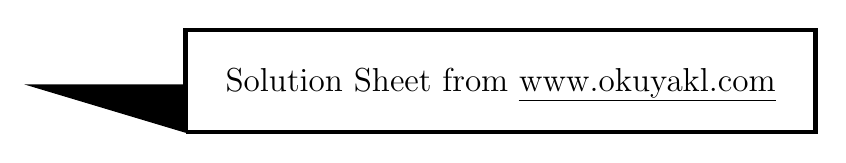
\begin{tikzpicture}(10,3)
		\draw[ultra thick](2,0) --(10,0) -- (10,1.3) --(2,1.3) -- (2,0);
		\draw[fill=black](2,0)-- (0,.6) -- (2,.6) -- (2,0);
		\node at (6,.6) {\large Solution Sheet from \href{http://www.okuyakl.com}{www.okuyakl.com}};
	\end{tikzpicture}
	\vspace{0.5 cm}
	
	\noindent {\bf Task 1. a)}\\
	We solve the volume formula for this prism for $e$:
	$$
	\renewcommand{\arraystretch}{2}
	\begin{array}{rcll}
		V &=& G \cdot h \\
		V &=& {1 \over 2} e \cdot f \cdot h &|:f \quad |:h \quad |\cdot 2\\
		{2 V \over f \cdot h} &=& e
	\end{array}
	$$
	
	\noindent {\bf Task 1. b)}\\
	We insert the given values:
	$${ 2 \cdot 25.5 \over 4.3 \cdot 6.6} = \SI{1.80}{\centi \meter}$$
	
	\noindent {\bf Task 2.}\\
	We are proceeding step by step. First we calculate the hexagon area. It consists of six equilateral triangles with side length $\SI{6}{\centi\meter}$. Then the area of a triangle is:
	$$A_D={1\over 2} \cdot a \cdot b \cdot \sin\gamma = {1\over 2}\cdot 6^2 \cdot \sin 60^\circ = 9\sqrt{3} = \SI{15.59}{\centi\meter^2}$$
	The volume of the hexagonal prism is then:
	$$V_{Pr}=6\cdot A_D \cdot h = 6 \cdot 9 \cdot \sqrt{3} \cdot 23 = \SI{2151,21}{\centi\meter^3}$$
	The volume of the full glass cylinder is:
	$$V_{Z}=\pi r^2 \cdot h = \pi \cdot 7^2 \cdot 23 =\SI{3540.57}{\centi\meter}^3$$
	The weight of the remaining body is the difference between the cylinder and the prism multiplied by the density:
	$$ m = (3540.57-2151.21)\SI{}{\centi\meter^3} \cdot \SI{2,4}{\gram\per\centi\meter^3}=\SI{ 3334.47}{\gram}=\SI{3.33}{\kilogram}$$
	
	\noindent{\bf Task 3. a)}\\
	Using the Pythagorean theorem we calculate:
	$$
	\renewcommand{\arraystretch}{2}
	\begin{array}{rcll}
		\left({a\over 2}\right)^2 + h_k^2 & = & h_a^2 & | - h_k^2 \\
		\left({a\over 2}\right)^2 & = & h_a^2 - h_k^2 &| \sqrt{\qquad}\\
		{a\over 2} & = & \sqrt{h_a^2 - h_k^2} &|\cdot 2 \\
		a & = & 2 \cdot \sqrt{(\SI{9,4}{\centi\meter})^2-(\SI{7,8}{\centi\meter})^2} & = \SI {10.5}{\centi\meter}
	\end{array}
	$$
	The side edge is calculated with:
	$$
	\renewcommand{\arraystretch}{2}
	\begin{array}{rcll}
		s^2 & = & \left({a\over 2}\right)^2 + h_a^2 & | \sqrt{\qquad} \\
		s & = & \sqrt{(\SI{5,25}{\centi\meter})^2 + (\SI{9,4}{\centi\meter})^2} & =\SI{10, 77}{\centi\meter}
	\end{array}
	$$
	For the pyramid volume we get:
	$$V={1\over 3} \cdot a^2 \cdot h_k= {1\over 3} \cdot (\SI{10,5}{\centi\meter})^2 \cdot \SI{7 .8}{\centi\meter} = \SI{286.7}{\centi\meter^3}$$
	The lateral surface consists of four isosceles triangles:
	$$M=4\cdot {1\over 2} a \cdot h_a= 2\cdot \SI{10,5}{\centi\meter} \cdot \SI{9,4}{\centi\meter} = \SI{197.4}{\centi\meter^2}$$
	To get the entire surface, we add the base area:
	$$O = M + a^2 = \SI{197.4}{\centi\meter^2}+(\SI{10.5}{\centi\meter})^2 = \SI{307.7 }{\centi\meter^2}$$
	
	\noindent{\bf Task 3. b)}\\
	We use the Pythagorean theorem again:
	$$
	\renewcommand{\arraystretch}{2}
	\begin{array}{rcll}
		h_k^2 + \left({a\over 2}\right)^2 & = & h_a^2 &| -\left({a\over 2}\right)^2 \\
		h_k^2 & = & h_a^2 - \left({a\over 2}\right)^2 & | \sqrt{\qquad}\\
		h_k & = & \sqrt{(\SI{18}{\centi\meter})^2 - (\SI{7.5}{\centi\meter})^2} & = \SI{16.4} {\centi\meter}\\
	\end{array}
	$$
	The following applies to the side edge $s$:
	$$s=\sqrt{\left({a\over 2}\right)^2 + h_a^2}= \sqrt{(\SI{7.5}{\centi\meter})^2 + (\SI{18}{\centi\meter})^2 } = \SI{19.5}{\centi\meter}$$
	We calculate the volume with:
	$$V={1\over 3} \cdot a^2 \cdot h_k= {1\over 3} \cdot (\SI{15}{\centi\meter})^2 \cdot \SI{16,4 }{\centi\meter} = \SI{1230}{\centi\meter^3}$$
	The lateral surface consists of four isosceles triangles:
	$$M=4\cdot {1\over 2} a \cdot h_a= 2\cdot \SI{15}{\centi\meter} \cdot \SI{18}{\centi\meter} = \SI{540 }{\centi\meter^2}$$
	To get the entire surface, we add the base area:
	$$O = M + a^2 = \SI{540}{\centi\meter^2}+(\SI{15}{\centi\meter})^2 = \SI{765}{\centi\meter ^2}$$
	
	\begin{center}
		\includegraphics[width=7 cm]{../../viecher/eendcomic.pdf}
		
		Here you can go back to the \href{https://www.okuyakl.de/math/m9korL046/ae046.pdf}{task sheet}
	\end{center}
	
	
\end{document}